\documentclass{beamer}
\usepackage[orientation=portrait,size=a0,scale=1.2]{beamerposter}
\usepackage{haziq_poster_portrait}
\usepackage{haziq_maths}

%%%%%%%%%%%%%%%%%%%%%%%%%%%%%%%%%%%%%%%%%%%%%%%%%%%%%%%%%%%%%%%%%%%%%%%%%%%%%%%%
%%% POSTER SETTINGS %%%%%%%%%%%%%%%%%%%%%%%%%%%%%%%%%%%%%%%%%%%%%%%%%%%%%%%%%%%%
%%%%%%%%%%%%%%%%%%%%%%%%%%%%%%%%%%%%%%%%%%%%%%%%%%%%%%%%%%%%%%%%%%%%%%%%%%%%%%%%
\setbeamercolor{block title}{fg=black,bg=white}
\setbeamercolor{block body}{fg=black,bg=white}
\setbeamercolor{block alerted title}{fg=white,bg=black}
\setbeamercolor{block alerted body}{fg=black,bg=white}

% Define the column widths and overall poster size
% To set effective sepwid, onecolwid and twocolwid values, first choose how many columns you want and how much separation you want between columns
% In this template, the separation width chosen is 0.024 of the paper width and a 4-column layout
% onecolwid should therefore be (1 - sepwid * (# of columns + 1)) / # of columns 
% e.g. (1 - 0.024 * (4 + 1)) / 4 = 0.22
% Set twocolwid to be (2 * onecolwid) + sepwid = 0.464
% Set threecolwid to be (3 * onecolwid) + 2 * sepwid = 0.708
% The whole poster consists of three major columns, the second of which is split into two columns twice - the [t] option aligns each column's content to the top
% A0 is 1189 x 841 mm
% A1 is 594 x 841 mm
% sep      =  28.536 mm
% half sep =  14.268 mm
% onecol   = 261.580 mm
% total    = 304.384 mm
\newlength{\sepwid}
\newlength{\onecolwid}
\newlength{\twocolwid}
\newlength{\threecolwid}
\setlength{\sepwid}{0.03\paperwidth} % Separation width (white space) between columns
\setlength{\onecolwid}{0.2933\paperwidth} % Width of one column
\setlength{\twocolwid}{0.6167\paperwidth} % Width of two columns
\setlength{\threecolwid}{0.9400\paperwidth} % Width of three columns

% Title section
\title{
  \vspace{0.3ex}
  Binary and Multinomial Regression\\[0.4ex]
  and Classification using I-priors
}

\author{Haziq Jamil \&\\[-0.4ex] Wicher Bergsma}

\institute{
  ~\\[-1.9ex]
  Department of Statistics\\
  London School of Economics and\\
  Political Science\\[0.4ex]
  \url{https://phd.haziqj.ml}
}

%%%%%%%%%%%%%%%%%%%%%%%%%%%%%%%%%%%%%%%%%%%%%%%%%%%%%%%%%%%%%%%%%%%%%%%%%%%%%%%%
%%% BEGIN DOCUMENT %%%%%%%%%%%%%%%%%%%%%%%%%%%%%%%%%%%%%%%%%%%%%%%%%%%%%%%%%%%%%
%%%%%%%%%%%%%%%%%%%%%%%%%%%%%%%%%%%%%%%%%%%%%%%%%%%%%%%%%%%%%%%%%%%%%%%%%%%%%%%%
\begin{document}
\begin{frame}[t]  % the whole poster is enclosed in one beamer frame
\vspace{-35pt}  % shift everything up closer to the line
\begin{columns}[t]  % and in the columns environment

%%%%%%%%%%%%%%%%%%%%%%%%%%%%%%%%%%%%%%%%%%%%%%%%%%%%%%%%%%%%%%%%%%%%%%%%%%%%%%%%
%%% SET UP THREE COL WIDTH %%%%%%%%%%%%%%%%%%%%%%%%%%%%%%%%%%%%%%%%%%%%%%%%%%%%%
%%%%%%%%%%%%%%%%%%%%%%%%%%%%%%%%%%%%%%%%%%%%%%%%%%%%%%%%%%%%%%%%%%%%%%%%%%%%%%%%
% Everything is in a 3-column wide column
\spacercolumn
\begin{column}{\threecolwid}
\begin{columns}[t,totalwidth=\threecolwid]  % split the 3-col

%%%%%%%%%%%%%%%%%%%%%%%%%%%%%%%%%%%%%%%%%%%%%%%%%%%%%%%%%%%%%%%%%%%%%%%%%%%%%%%%
%%% FIRST COLUMN %%%%%%%%%%%%%%%%%%%%%%%%%%%%%%%%%%%%%%%%%%%%%%%%%%%%%%%%%%%%%%%
%%%%%%%%%%%%%%%%%%%%%%%%%%%%%%%%%%%%%%%%%%%%%%%%%%%%%%%%%%%%%%%%%%%%%%%%%%%%%%%%
\begin{column}{\onecolwid}  % start first column

% Keywords ---------------------------------------------------------------------
\begin{figure}[t]
  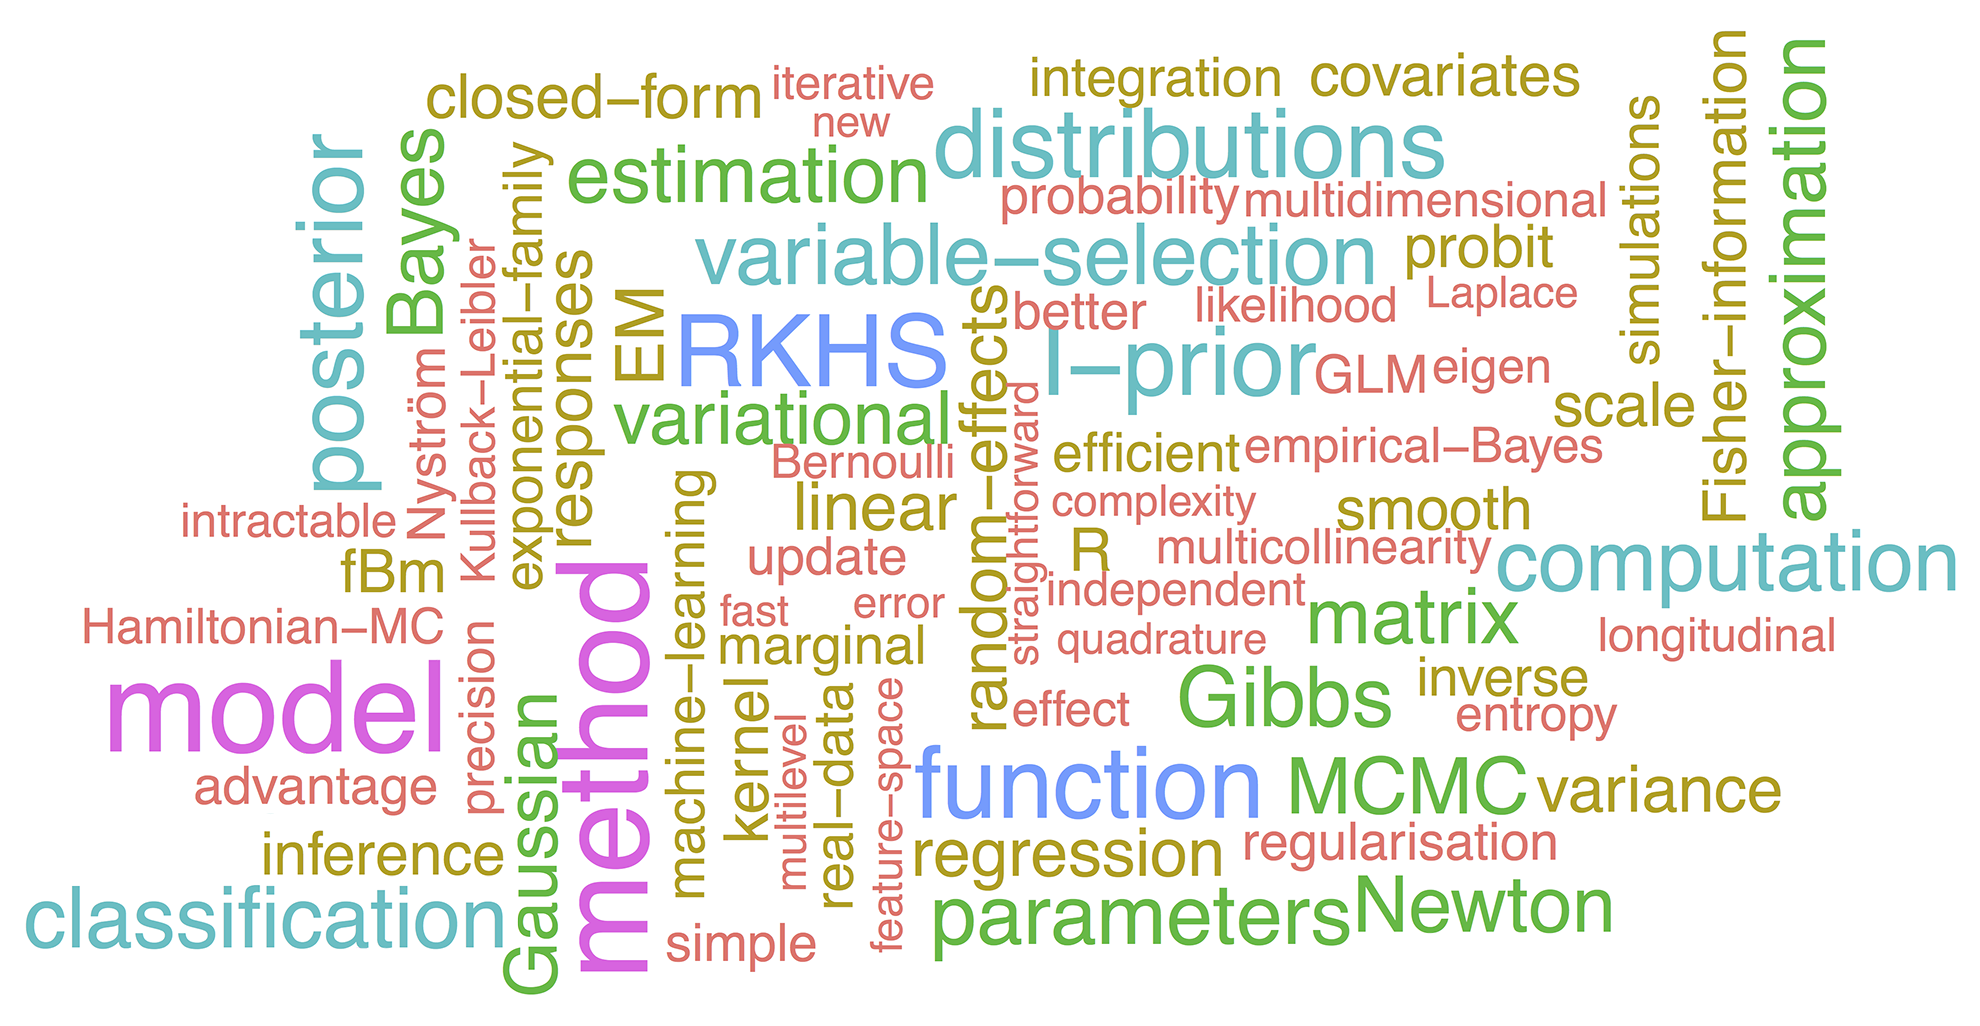
\includegraphics[width=\linewidth]{figure/keyword.png}
\end{figure}

% Introduction -----------------------------------------------------------------
\begin{block}{Introduction}

Consider the regression model for $i=1,\dots,n$:
~\\[-21pt]
\begin{align}\label{eq:normalmodel}
  \begin{gathered}
      y_i = \alpha + f(x_i) + \epsilon_i \\
    (\epsilon_1, \dots, \epsilon_n)^\top \sim \N_n(0,\Psi^{-1})
  \end{gathered}
\end{align}
~\\[-7pt]
where $y_i \in \bbR$, $x \in \cX$, $f \in \cF$ and $\alpha\in\bbR$ is an intercept. 
Let $\cF$ be a reproducing kernel Hilbert space (RKHS) with kernel $h_\lambda:\cX \times \cX \to \bbR$. 
The Fisher information for $f$ evaluated at $x$ and $x'$ is
~\\[-22pt]
\begin{align}
  \cI\big(f(x), f(x')\big) = \sum_{k=1}^n \sum_{l=1}^n \Psi_{k,l} h_\lambda(x,x_k) h_\lambda(x',x_l).
\end{align}

\setbeamercolor{block alerted title}{fg=white,bg=colgrey} % Change the alert block title colors
\setbeamercolor{block alerted body}{fg=black,bg=white} % Change the alert block body colors
\begin{alertblock}{The I-prior}
\vspace{3pt}
The entropy maximising prior distribution for $f$, subject to identifiability constraints, is 
~\\[-13pt]
\[
  \bff = \big(f(x_1),\dots,f(x_n) \big)^\top \sim \N_n \big(\bff_0, \cI[f] \big).
\]
~\\[-18pt]
Equivalently, $f(x) = f_0(x) + \sum_{i=1}^n h_\lambda(x,x_i)w_i$, with
~\\[-13pt]
\[
  (w_1, \dots, w_n)^\top \sim \N_n(0,\Psi).
\]
\vspace{-11pt}

\end{alertblock}

\vspace{-10pt}
Of interest are 

\newcommand{\new}{{\text{new}}}
\begin{itemize}
  \item the posterior distribution for the regression function
  \vspace{-10pt}
  \[
    p(\bff|\by) = \frac{p(\by|\bff) p(\bff)}{\int p(\by|\bff) p(\bff) \d \by}; \text{and}
  \]
  \vspace{-16pt}
  \item the posterior predictive distribution for new data points
  \[
    p(y_\new|\by) = \int p(y_\new|f_\new,\by) p(f_\new|\by) \d f_\new.
  \]
\end{itemize}
\vspace{5pt}
Model parameters (error precision $\Psi$, RKHS scale parameters $\lambda$, and any other kernel parameters) may need to be estimated.
%, e.g. using likelihood methods or even MCMC.

\end{block}

% A Unifying Regression --------------------------------------------------------
\begin{block}{A Unified Regression Framework}

\begin{itemize}
%  \setlength\itemsep{0.3em}
  \item Multiple linear regression (canonical RKHS)
  \item Smoothing models (fBm RKHS)
  \item Multilevel regression (ANOVA RKHS: canonical \& Pearson)
  \vspace{3pt}
  \[
      f(x_i^{(j)}) = f_1(j) + f_2(x_i^{(j)}) + f_{12}(x_i^{(j)}, j)
  \]
  \vspace{-35pt}  
  \item Longitudinal modelling (ANOVA RKHS: fBm \& Pearson)
  \vspace{3pt}
  \[
    f(x_i, t_i) = f_1(t_i) + f_2(x_{i}) + f_{12}(x_{i},t_i)
  \]
  \vspace{-34pt}
  \item Functional covariates ($\cX$ a Hilbert-Sobolev space)
\end{itemize}

\end{block}

\end{column}  % end of first column

%%%%%%%%%%%%%%%%%%%%%%%%%%%%%%%%%%%%%%%%%%%%%%%%%%%%%%%%%%%%%%%%%%%%%%%%%%%%%%%%
%%% FIGURE SPANNING COLS 2-3 %%%%%%%%%%%%%%%%%%%%%%%%%%%%%%%%%%%%%%%%%%%%%%%%%%%
%%%%%%%%%%%%%%%%%%%%%%%%%%%%%%%%%%%%%%%%%%%%%%%%%%%%%%%%%%%%%%%%%%%%%%%%%%%%%%%%
\begin{columns}[t,totalwidth=\twocolwid]  % set up 2-col width
\begin{column}{\twocolwid}

% I-prior figures --------------------------------------------------------------
\begin{figure}
\includegraphics[width=0.33\linewidth]{figure/kernel_path_canonical}
\includegraphics[width=0.33\linewidth]{figure/kernel_path_fbm}
\includegraphics[width=0.33\linewidth]{figure/kernel_path_pearson}
\vspace{-40pt}
\caption{(L-R) Sample I-prior paths from the canonical (linear), fractional Brownian motion (fBm), and Pearson RKHS. The (reproducing) kernels corresponding to each RKHS are $h_\lambda(x,x') = \lambda  \langle x,x' \rangle_\cX$ (linear), $h_\lambda(x,x') = -\frac{\lambda}{2} \big( \norm{x-x'}_\cX^{2\gamma} - \norm{x}_\cX^{2\gamma} - \norm{x'}_\cX^{2\gamma}\big)$ (fBm), and $h_\lambda(x,x') = \lambda \big( {\delta_{xx'}} / {\Prob[X=x]} - 1 \big)$ (Pearson).}
\end{figure}

%%%%%%%%%%%%%%%%%%%%%%%%%%%%%%%%%%%%%%%%%%%%%%%%%%%%%%%%%%%%%%%%%%%%%%%%%%%%%%%%
%%% SECOND COLUMN %%%%%%%%%%%%%%%%%%%%%%%%%%%%%%%%%%%%%%%%%%%%%%%%%%%%%%%%%%%%%%
%%%%%%%%%%%%%%%%%%%%%%%%%%%%%%%%%%%%%%%%%%%%%%%%%%%%%%%%%%%%%%%%%%%%%%%%%%%%%%%%
\begin{columns}[t,totalwidth=\twocolwid]  % split the 2-col width in two
\begin{column}{\onecolwid}

% Categorical responses --------------------------------------------------------
\begin{block}{Categorical Responses}
\vspace{2pt}

When each $y_i \in \{ 1,\dots,m \}$, normality assumptions are violated.
Model instead $y_i = \argmax_k y_{ik}^*\,$, where %for $j=1,\dots,m$,
~\\[-18pt]
\begin{align}\label{eq:iprobit}
  \begin{gathered}
    y_{ij}^* = \alpha_j + f_j(x_i) + \epsilon_{ij} \\    
%    \text{vec}\left( \epsilon_{ij} \right)_{i,j} \sim \N_{nm}\big(0, \Sigma \otimes \Psi^{-1}\big)
    (\epsilon_{i1},\dots,\epsilon_{im})^\top \sim \N_m(0, \Sigma) \\
  \end{gathered}
\end{align}
~\\[-5pt]
with $\Cov(\epsilon_{ij},\epsilon_{kj}) = 0$, for all $i\neq k$, $j=1,\dots,m$.
In other words, $\Psi$ is diagonal in (1) and (2). 
The I-prior is
~\\[-18pt]
\begin{align*}
  \begin{gathered}
    \bff_j = \big(f_j(x_1),\dots,f_j(x_n) \big)^\top \sim \N_n \big(\bff_{0j}, \Sigma^{-1}_{jj}\cdot\cI[f] \big) \\[0.5ex]
    \Cov( \bff_j, \bff_k) = \Sigma^{-1}_{jk} \cdot\cI[f].
  \end{gathered}
\end{align*}
~\\[-5pt]
Class probabilities $p_{ij}$ are obtained using a \emph{conically truncated $m$-variate normal} density
~\\[-14pt]
\[
  p_{ij} = 
%  \int \ind\left[\{y_{ij}^* > y_{ik}^* | k \neq j \} \right] \cdot 
  \hspace{-1.3cm}
  \mathop{\int}_{\{y_{ij}^* > y_{ik}^* \,|\, k \neq j \}}
  \hspace{-1.3cm}
  \N_m\big(\by^*_i \,|\, \bff(x_i),\Sigma\big) \d\by_i^* \, =: \, g_j^{-1}\big(\bff(x_i)\big).
\]
~\\[-9pt]
where we had defined $\bff(x_i) = \big(f_1(x_i),\dots,f_m(x_i)\big)^\top$.
Now, the marginal, on which the posterior depends,
~\\[-12pt]
\[
  p(\by) = \hspace{-9pt} \int \hspace{-4pt} \prod_{i,j} \hspace{-2pt} \Big\{ g_j^{-1}\big(\bff(x_i)\big) \hspace{-5pt} \Big\}^{[y_i = j]} \hspace{-10pt}\cdot\hspace{-3pt} \N_{nm}\big(\bff \;\!|\;\! \bff_{0}, \Sigma \otimes \cI[f]\big) \d \bff ,
\]
~\\[-4pt]
cannot be found in closed form.
By working in a fully Bayesian setting, we append model parameters and employ a \emph{variational approximation}.
 
\end{block}

% Spatio-temporal modelling of BTB ---------------------------------------------
\begin{block}{Spatio-Temporal Modelling of BTB\textsuperscript{a}}
\vspace{2pt}

Determine the existence of spatial segregation of the different spoligotypes of bovine tuberculosis (BTB) in Cornwall, UK, and whether the spatial distribution had changed over time.

\begin{enumerate}
  \item Constant model (constant RKHS)
  \vspace{5pt}
  \[
    p_{ij} = g^{-1}_j\big( \alpha_k \big)_{k=1}^m
  \]
  \vspace{-32pt}
  \item Spatial segregation (fBm RKHS)
  \vspace{3pt}
  \[
    p_{ij} = g^{-1}_j\big(\alpha_k + f_{1k}(x_i) \big)_{k=1}^m
  \]
  \vspace{-34pt}  
  \item Spatio-temporal segregation (ANOVA RKHS)
  \vspace{6pt}
  \[
    p_{ij} = g^{-1}_j\big(\alpha_k + f_{1k}(x_i) + f_{2k}(t_i) + f_{12k}(x_i,t_i) \big)_{k=1}^m
  \]
  \vspace{-38pt}
\end{enumerate}  

Evidence Lower Bound (ELBO) values for the three models are -1197.4, -665.3, and -656.2 respectively.
% -656.2  spatio-temporal
% -664.7  spatio-period
\end{block}


\end{column}

%%%%%%%%%%%%%%%%%%%%%%%%%%%%%%%%%%%%%%%%%%%%%%%%%%%%%%%%%%%%%%%%%%%%%%%%%%%%%%%%
%%% THIRD COLUMN %%%%%%%%%%%%%%%%%%%%%%%%%%%%%%%%%%%%%%%%%%%%%%%%%%%%%%%%%%%%%%%
%%%%%%%%%%%%%%%%%%%%%%%%%%%%%%%%%%%%%%%%%%%%%%%%%%%%%%%%%%%%%%%%%%%%%%%%%%%%%%%%
\begin{column}{\onecolwid}

% Detecting Cardiac Arrhythmia -------------------------------------------------
\begin{block}{Detecting Cardiac Arrhythmia\textsuperscript{b}}
\vspace{2pt}
  
Predict whether or not patients suffer from a cardiac disease based on various patient profiles such as age, height, weight and a myriad of electrocardiogram (ECG) readings ($p=271, n=451$).  
  
\end{block}

\vspace{-21pt}
\begin{table}
  \caption{Mean out-of-sample misclassification rates and standard errors for 100 runs of various training ($s$) and test ($451-s$) sizes for the cardiac arrhythmia binary classification task.}
  \vspace{47pt}
  \small
  \begin{tabular}{l r r r}
  \toprule
  &\multicolumn{3}{ c }{\textbf{Misclassification rate (\%)}} \\
  \textbf{Method\hspace{40mm}}
  & \hspace{0.5cm} \textbf{\hspace{11mm}\boldmath$s = 50$} 
  & \hspace{0.5cm} \textbf{\hspace{11mm}\boldmath$s = 100$} 
  & \hspace{0.5cm} \textbf{\hspace{11mm}\boldmath$s = 200$} \\
  \midrule
  {I-probit (linear)}  & 34.5 (0.4) & 31.4 (0.4) & 29.7 (0.4) \\
  {I-probit (fBm)}     & 34.7 (0.6) & 27.3 (0.3) & 24.5 (0.3) \\[0.5em]
  {GP (Gaussian)}      & 37.3 (0.4) & 33.8 (0.4) & 29.3 (0.4) \\  
  {L-1 logistic}       & 34.9 (0.4) & 30.5 (0.3) & 26.1 (0.3) \\[0.5em] 
  {SVM (linear)}       & 36.2 (0.5) & 35.6 (0.4) & 35.2 (0.4) \\
  {SVM (Gaussian)}     & 48.4 (0.5) & 47.2 (0.5) & 46.9 (0.4) \\[0.5em] 
  {RF}                 & 31.7 (0.4) & 26.7 (0.3) & 22.4 (0.3) \\
  {$k$-NN}             & 40.6 (0.3) & 38.9 (0.3) & 35.8 (0.4) \\
  \bottomrule
  \end{tabular}
\end{table}  

%  {I-probit (linear)}  & 34.5 (0.43) & 31.4 (0.38) & 29.7 (0.35) \\
%  {I-probit (fBm)}     & 34.7 (0.59) & 27.3 (0.29) & 24.5 (0.30) \\[0.5em]
%  {GP (Gaussian)}      & 37.3 (0.42) & 33.8 (0.40) & 29.3 (0.35) \\  
%  {L-1 logistic}       & 34.9 (0.42) & 30.5 (0.34) & 26.1 (0.27) \\[0.5em] 
%  {SVM}                & 36.2 (0.47) & 35.6 (0.39) & 35.2 (0.35) \\
%  {RF}                 & 31.7 (0.39) & 26.7 (0.29) & 22.4 (0.31) \\[0.5em] 
%  {$k$-NN}             & 40.6 (0.33) & 38.9 (0.33) & 35.8 (0.36) \\

% Conclusion -------------------------------------------------------------------
\vspace{20pt}
\setbeamercolor{block alerted title}{fg=white,bg=colgrey} % Change the alert block title colors
\setbeamercolor{block alerted body}{fg=black,bg=white} % Change the alert block body colors
\begin{alertblock}{Conclusions}

\begin{itemize}
  \item Simple estimation of various categorical models:
  \begin{itemize}
    \item Choice models (with or without IIA);
    \item Random-effects models;
    \item Binary and multiclass classification.
  \end{itemize}
  \item Inference is straightforward (e.g. model com- parison or (transformed) credibility intervals).
  \item Great predictive abilities.
\end{itemize}

\end{alertblock}

% References -------------------------------------------------------------------
\vspace{4pt}
\begin{block}{References}

\vspace{-18pt}
\nocite{*}
\bibliographystyle{unsrt}
\small{\bibliography{bib/phd-poster}}

\end{block}

\end{column}  % end of third column

%%%%%%%%%%%%%%%%%%%%%%%%%%%%%%%%%%%%%%%%%%%%%%%%%%%%%%%%%%%%%%%%%%%%%%%%%%%%%%%%
%%% END OF THREE COL WIDTH %%%%%%%%%%%%%%%%%%%%%%%%%%%%%%%%%%%%%%%%%%%%%%%%%%%%%
%%%%%%%%%%%%%%%%%%%%%%%%%%%%%%%%%%%%%%%%%%%%%%%%%%%%%%%%%%%%%%%%%%%%%%%%%%%%%%%%
\end{columns}  % end of 2-col split
\end{column}
\end{columns}  % end of 2-col caused by figure span 2-3
\end{columns}  % end of 3-col split

%%%%%%%%%%%%%%%%%%%%%%%%%%%%%%%%%%%%%%%%%%%%%%%%%%%%%%%%%%%%%%%%%%%%%%%%%%%%%%%%
%%% FIGURE SPANNING THREE COLUMNS %%%%%%%%%%%%%%%%%%%%%%%%%%%%%%%%%%%%%%%%%%%%%%
%%%%%%%%%%%%%%%%%%%%%%%%%%%%%%%%%%%%%%%%%%%%%%%%%%%%%%%%%%%%%%%%%%%%%%%%%%%%%%%%

% BTB plots --------------------------------------------------------------------
\vspace{-15pt}
\begin{figure}
%  \includegraphics[width=0.246\linewidth]{figure/btb_st_1}
%  \includegraphics[width=0.246\linewidth]{figure/btb_st_2}
%  \includegraphics[width=0.246\linewidth]{figure/btb_st_3}
%  \includegraphics[width=0.246\linewidth]{figure/btb_st_4}
  \includegraphics[width=0.246\linewidth]{figure/btb_spat_4}
  \includegraphics[width=0.246\linewidth]{figure/btb_spat_2}
  \includegraphics[width=0.246\linewidth]{figure/btb_spat_3}
  \includegraphics[width=0.246\linewidth]{figure/btb_spat_1}  
  \vspace{-9pt}
  \caption{Predicted probability surfaces for BTB contraction in Cornwall for the four largest spoligotypes of the bacterium \emph{Mycobacterium bovis} over the entire time period 1989--2002 using Model 2.}
\end{figure}

\vspace{30pt}
{\small\color{black!65} Data sources: \textsuperscript{a}Peter Diggle, Pingping Zheng, and Peter Durr. Nonparametric estimation of spatial segregation in a multivariate point process: bovine tuberculosis in Cornwall, UK. \emph{J. Royal Stat. Soc. Series C (Appl. Statist.)}, 54(3):645--658, 2005.
\textsuperscript{b}Timothy I Cannings and Richard J Samworth. Random projection ensemble classification. \emph{J. Royal Stat. Soc. Series B (Stat. Methodol.)}, 79(4):959--1035, 2017.}

\end{column}  % end of overall 3-col column

%%%%%%%%%%%%%%%%%%%%%%%%%%%%%%%%%%%%%%%%%%%%%%%%%%%%%%%%%%%%%%%%%%%%%%%%%%%%%%%%
%%% END DOCUMENT %%%%%%%%%%%%%%%%%%%%%%%%%%%%%%%%%%%%%%%%%%%%%%%%%%%%%%%%%%%%%%%
%%%%%%%%%%%%%%%%%%%%%%%%%%%%%%%%%%%%%%%%%%%%%%%%%%%%%%%%%%%%%%%%%%%%%%%%%%%%%%%%
\spacercolumn
\end{columns}  % end of all the columns in the poster

% Draw lines separating columns
\tikz[remember picture,overlay]{\draw[black, ultra thick] ([shift={(0.3383\paperwidth,-13cm)}]current page.north west) -- ([shift={(0.3383\paperwidth,27cm)}]current page.south west);}
\tikz[remember picture,overlay]{\draw[black, ultra thick] ([shift={(-0.3383\paperwidth,-35cm)}]current page.north east) -- ([shift={(-0.3383\paperwidth,27cm)}]current page.south east);}
\tikz[remember picture,overlay]{\draw[black, thick] ([shift={(0.0212\paperwidth,120pt)}]current page.south west) -- ([shift={(8cm,120pt)}]current page.south west);}
%\tikz[remember picture,overlay]{\draw[black,ultra thick] ([shift={(0,0.0212\paperwidth)}]current page.south east) -- ([shift={(0,0.0212\paperwidth)}]current page.south west);}  % bottom guide

\end{frame}  % end of the enclosing frame
\end{document}
